\documentclass[12pt,a4paper]{article}
\usepackage[utf8]{inputenc}
\usepackage[english,lithuanian]{babel}
\usepackage[L7x]{fontenc}
\usepackage{lmodern}
\usepackage{amsmath}
\usepackage{amssymb}
\usepackage{theorem}
\usepackage{bm}
\usepackage{Sweave}
%\usepackage[unicode]{hyperref}
%\usepackage{ucshyper}
\pagestyle{plain}

\newcommand{\eps}{\varepsilon}
\newcommand{\E}{\mathbf{E}}
\newcommand{\PP}{\mathbf{P}}
\theoremstyle{change}\newtheorem{salyga}{Uždavinys}

\DeclareMathOperator{\spp}{sp}

\DeclareMathOperator{\Corr}{Corr}
\topmargin=0cm
\textheight=700pt
\textwidth=430pt
\oddsidemargin=0pt
\headsep=0pt
\headheight=0pt
%\voffset=-1in
\def\qed{\relax\ifmmode\hskip2em \Box\else\unskip\nobreak\hskip1em $\Box$\fi}

\begin{document}
\begin{titlepage}
\centerline{ \large VILNIAUS UNIVERSITETAS}
\bigskip
\centerline{\large MATEMATIKOS IR INFORMATIKOS FAKULTETAS}
\smallskip

\centerline{\large  EKONOMETRINĖS ANALIZĖS KATEDRA}
\vskip 200pt
\centerline{ \large Alina \textsc{Rauktytė} ir Povilas \textsc{Bočkus}}
\vskip 50pt
\centerline{\Large Ekonometrinio projekto}
\vskip 25pt
\centerline{\bf \Large \textsc{Darbo užmokesčio nustatymo mechanizmas}}
\vskip 25pt
\centerline{\Large Pradinė duomenų analizė}
\bigskip
\vskip 50pt
\begin{flushright}
 Kursinio projekto vadovas: 
 doc. Remigijus Lapinskas
\end{flushright}
\hfill Ekonometrija, III kursas, 2 grupė
\vskip 150pt
\centerline{\large VILNIUS 2011}
\end{titlepage}



\
Mūsų nagrinėjama tema “Darbo užmokesčio nustatymo mechanizmas” apima šiuos Lietuvos ekonominę padėtį ir 
darbo rinką nusakančius duomenis (duomenų šaltinis http://www.stat.gov.lt/lt/):

\medskip
\begin{itemize}

\item Wage – vidutinis nominalusis atlyginimas;
\item L – darbo jėga;
\item P – vartotojų kainų indeksas;
\item E -  darbuotojų skaičius;
\item GDP – bendras vidaus produktas.

\end{itemize}
Visi aukščiau minėti duomenys yra nuo 2000 – ųjų metų pirmojo ketvirčio iki 2008 – ųjų metų ketvirto ketvirčio imtinai.
\vskip 0pt
$\quad$ Darbo užmokestis yra tema, plačiai nagrinėjama ekonomistų. Mūsų pagrindinis tikslas yra ištirti, kaip darbo užmokestis Lietuvoje priklauso nuo tokių ekonomikos faktorių kaip kainų lygis, bendras vidaus produktas ir kintamųjų atspindinčių užimtumą ir darbo jėgą. Iš gausybės ekonominių modelių, tiriančių darbo užmokesčio priklausomybę nuo minėtų kintamųjų, pasirinkome šiuos: darbo užmokesčio priklausomybė nuo paties savęs (nuo Wage laikinės sekos ankstinių) ir regresijos modelis įtraukiant paklaidų korekcijos narį. 

\vskip 0pt
$\quad$Toliau ištirsime kiekvieną kintamąjį detaliau. 



\begin{flushleft}
\textbf{\Large {Nominalusis atlyginimas (wage)}}
\end{flushleft}
\vskip 15pt
$\quad$Nominalieji Lietuvos darbuotojų atlyginimai buvo gauti kaip trijų sektorių vidutinių atlyginimų vidurkis, t.y. kiekvienų metų ketvirčio, pradedant nuo 2000 – ųjų pirmojo ketvirčio ir baigiant 2008 – ųjų ketvirtu ketvirčiu, šalies ūkio be individualių įmonių, valstybės sektoriaus ir privataus sektoriaus be individualių įmonių atlyginimų bendras vidutinis atlyginimas.
\vskip 0pt
$\quad$ Mus domina, kokia yra Lietuvos atlyginimų dydžio tendencija laiko atžvilgiu. Pateikiame nominalaus atlyginimo grafiką:
\\
\begin{center}
\includegraphics[width=70mm,height=70mm]{nwage}
\end{center}
Iš grafiko matyti, kad vidutinis nominalusis atlyginimas eksponentiškai didėja, todėl duomenis išlogaritmavome. Išskirtys šiems duomenims nebūdingos. 

\begin{flushleft}
\textbf{\Large {Darbo jėga (L)}}
\end{flushleft}
\vskip 15pt
$\quad$ Darbo jėga - tai visi dirbantys ir aktyviai ieškantys darbo šalies piliečiai, kitaip tariant, žmonės, kurie nori ir gali dirbti, ir kurie dirba. Duomenyse darbo jėga matuojama tūkstančiais. 
\\
\begin{center}
\includegraphics[width=70mm,height=70mm]{l}
\end{center}
Grafike matoma darbo jėgos mažėjimo tendencija. Duomenys mažėja eksponentiškai, todėl naudosime darbo jėgos logaritmus. Ties 2003 metų 2 ketvirčiu matyti išskirtis.

\begin{flushleft}
\textbf{\Large {Vartotojų kainų indeksas (P)}}
\end{flushleft}
\vskip 15pt
$\quad$Kainų indekso baziniu laikotarpiu pasirinkti 2005 metai.
\\
\begin{center}
\includegraphics[width=70mm,height=70mm]{p}
\end{center}
Matome aiškią kainų kilimo tendenciją. Naudosime kainų indekso logaritmus, nes remiantis grafiku, duomenys auga eksponentiškai. Nuo 2000 metų iki 2004 metų kainų indeksas gana stabilus palyginti su kainų indekso elgesiu nuo 2004 metų,- nuo to laikotarpio kainų indekso kilimo greitis didėja. 

\begin{flushleft}
\textbf{\Large {Dirbančiųjų skaičius (E)}}
\end{flushleft}
\vskip 15pt
$\quad$Lietuvos dirbančiųjų skaičius mūsų duomenyse matuojamas tūkstančiais.
\\
\begin{center}
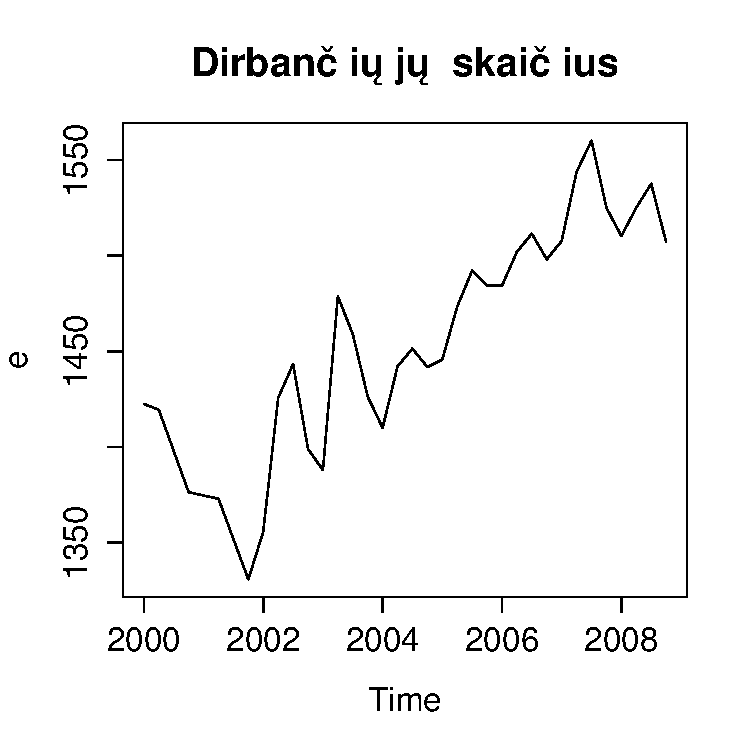
\includegraphics[width=70mm,height=70mm]{e}
\end{center}
Grafike matyti aiški dirbančiųjų skaičiaus augimo tendencija. 

\begin{flushleft}
\textbf{\Large {Bendras vidaus produktas (GDP)}}
\end{flushleft}
\vskip 15pt
$\quad$Nominalusis bendras vidaus produktas matuojamas milijonais. 
\\
\begin{center}
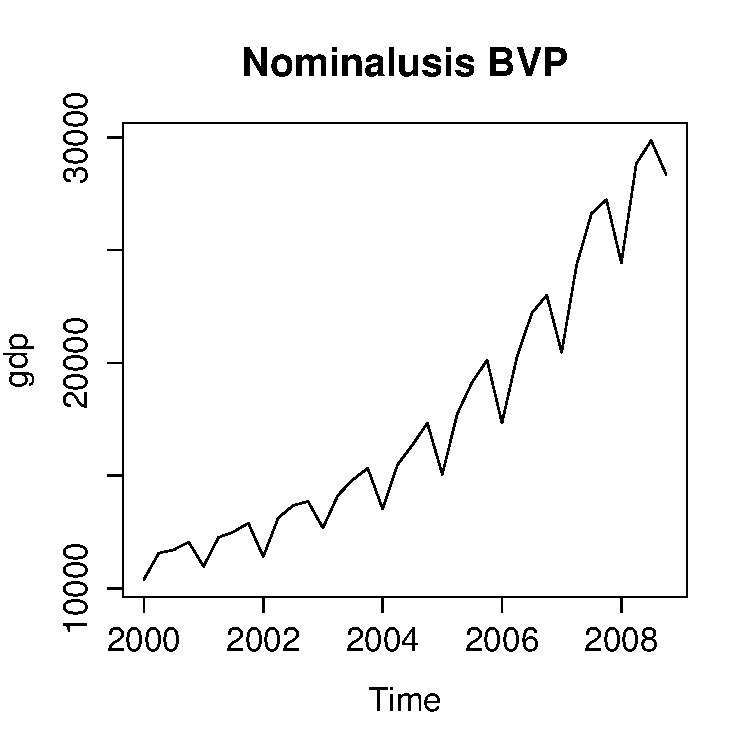
\includegraphics[width=70mm,height=70mm]{ngdp}
\end{center}
Grafike matyti aiški bendro šalies vidaus produkto augimo tendencija. Taip pat pastebimas ryškus BVP  duomenų sezoniškumas, todėl prieš įtraukiant kintamąjį į modelį, sezoniškumą panaikinsime. Dėl eksponentiško duomenų augimo, taip pat naudosime BVP logaritmus. 
\\
\begin{center}
\includegraphics[width=70mm,height=70mm]{gngdp}
\end{center}

\begin{flushleft}
\textbf{\Large {Kintamųjų vienetinių šaknų tyrimas}}
\end{flushleft}
\vskip 15pt

Vienetinės šaknies egzistavimo tyrimas reikalingas tam, kad galėtume tinkamai sudaryti kointegracijos modelį. Išsiaiškinsime, ar mūsų logaritmuoti duomenys turi vienetinę šaknį. Kiekvienam logaritmuotam kintamajam pritaikėme \textit{ur.df} funkciją norėdami ištirti vienetinės šaknies egzistavimą. Žemiau pateikiama lentelė su kiekvieno kintamojo statistikomis, gautomis \textit{ur.df} testu (kai $\alpha =0.05 $, kritinė reikšmė lygi –3.5).

\vskip 15pt

\begin{center}
\begin{tabular}{|c|c|}
\hline\textbf{ Kintamasis} &\textbf{ t - stat. reikšmė }\\ 
\hline log(wage) & -1.5776 \\ 
\hline log(L) & -2.0625 \\ 
\hline log(P) & -0.0441 \\ 
\hline log(E) & -2.9295 \\ 
\hline log(GDP) & -1.9487 \\ 
\hline 
\end{tabular} 
\end{center}
Kadangi visos t-statistikų reikšmės viršija kritinę reikšmę, nulinės hipotezės, kad egzistuoja vienetinė šaknis kiekviename iš kintamųjų, neatmetame. 










     
     
\end{document}